\chapter{Vision for Aircraft Manufacturing Automation}
\label{sec:VisionForAircraftManufacturingAutomation}

%%% Citation
{\small
\textit{"The problems of the world cannot possibly be solved by skeptics or cynics whose horizons are limited by the obvious realities. We need men who can dream of things that never were and ask why not?"}  -- \emph{John F. Kennedy}
%\begin{flushright}
%\emph{John F. Kennedy}
%\end{flushright}
}
\vspace{+10pt}
%%%%

This chapter illustrates robotic concepts to automate the manufacturing of large objects, such as airplanes, ships, buildings, etc. For those types of manufacturing tasks, unlike car production where the part can be on an assembly line and surrounded by robots, robots must be able to go inside the large manufactured object. %Additionally, with typically slower rates of production and larger numbers of distinct required operations, 


\section{Current situation}
\label{sec:CurrentSituation}

Here, the current manufacturing approach and the challenge for automating the manufacturing and assembly of aircraft is briefly explored.


\section{Solution Concepts}

Here, three class of possible solution are presented.




\subsection{Mobile climbing robots}
\label{sec:MobileClimbingRobots}

Another approach, aiming at a higher level of automation, is to have mobile robots walking or climbing inside the aircraft fuselage to reach manufacturing sites automatically. 


\begin{figure}[H]
	\centering
		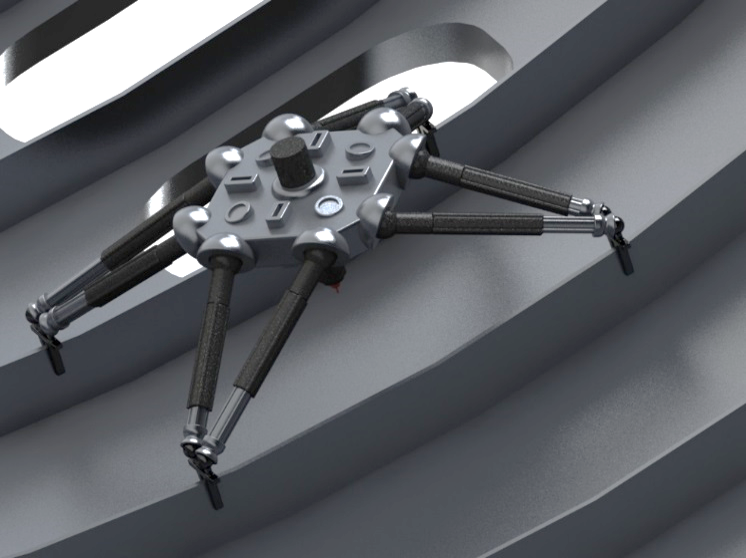
\includegraphics[width=0.9\textwidth]{spyder_concept.png}
		\caption{Mobile climbing manufacturing robot concept}
	\label{fig:arm_concept}
\end{figure}


\subsection{Wearable robots}
\label{sec:WearableRobots}

One possible solution, to solve bring robot on site easily is to use the help of humans, which unlike robot would have no problems navigating and moving inside a manufacturing site.

\begin{figure}[H]
	\centering
		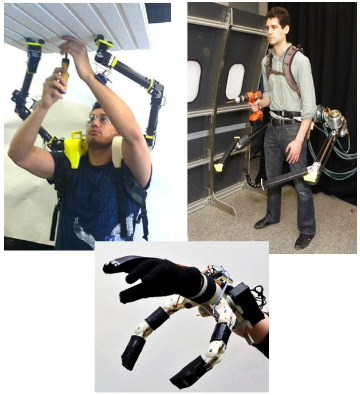
\includegraphics[width=0.6\textwidth]{wearables_robots.png}
		\caption{Wearable robot concepts and prototypes}
	\label{fig:wearable_concept}
\end{figure}


\subsection{Light-weight long manipulator arms}
\label{sec:LightWeightLongManipulatorArm}

Alternatively, robotic arm that would be very long and articulated could be able to reach manufacturing sites from the outside of the fuselage. 

\begin{figure}[H]
	\centering
		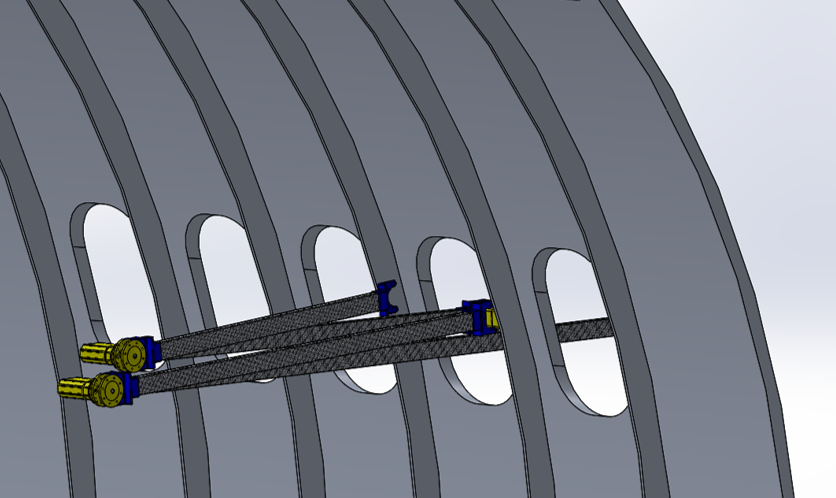
\includegraphics[width=1.00\textwidth]{arm_concept.png}
		\caption{Long light-weight arm concept for interior access}
	\label{fig:arm_concept}
\end{figure}